\section{The Belle II experiment}
The following sections introduce the \textbf{SuperKEKB} \cite{akai2018} collider, describing its technical setup briefly. It then presents the \textbf{Belle II} \cite{BelleIIPhysicsBook2019} detector discussing it sub-detector by sub-detector. Afterwards, the Belle II Analysis Software Framework (\textbf{basf2}) and \textbf{TopoAna} program are briefly described, with attention to the role of Monte Carlo methods in collider experiment simulation and reconstruction.

\subsection{The SuperKEKB collider}
\textbf{SuperKEKB} \cite{akai2018} is an asymmetric $e^+ e^-$ double-ring collider, located at KEK (The High Energy Accelerator Research Organization), in Tsukuba, Japan. It is the upgrade of the previous collider KEKB. It has a circumference of $3016$ m and collides bunches of electrons with bunches of positrons, respectively of energy 7 GeV (High Energy Ring -HER-) and 4 GeV (Low Energy Ring -LER-). Figure ~\ref{fig:superkekb_scheme} is a schematic image of the SuperKEKB design:

\begin{figure}[h]
    \centering
    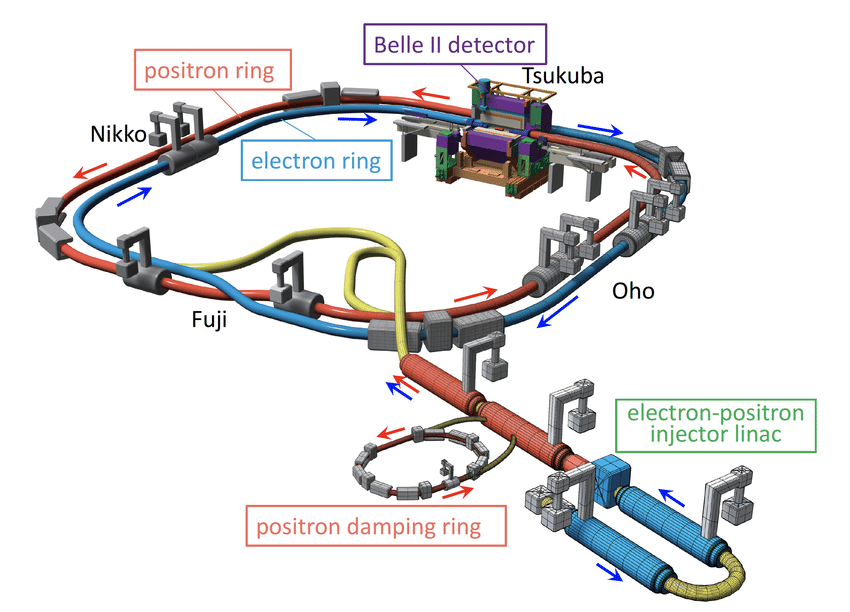
\includegraphics[width=1\textwidth]{belleII_det/images/superkekb.png}
    \caption{SuperKEKB design, where the Interaction Point (IP) is located in Tsukuba surrounded by the Belle II detector.}
    \label{fig:superkekb_scheme}
\end{figure}
It is noteworthy that the positron damping ring reduces the $e^+$ beam emittance, as positrons are obtained from a rotating tungsten target subjected. Electrons, by contrast, are injected directly from the linac since a controlled $e^-$ beam can easily be obtained \cite{kikuchi2005}.
$\\$
The resulting center-of-mass enrgy $\sqrt{s}$ in the IP can be modulated, but most of the data are acquired at the $\Upsilon(4S)$ resonance (10.58 GeV), an excited quarkonium state of $b \bar{b}$, which mainly decays into an entangled couple of $B\bar{B}$ ($\sim 100\%$). The $\Upsilon(4S)$ mass is just 20 MeV above the $B\bar{B}$ threshold, then the mesons are produced nearly in the rest frame. Since the lifetime of neutral B-mesons is short ($\tau = 1.510$ ps) and they are produced with low velocities, their path before decaying is short, making tough to separate the decays of the two produced mesons. The explicit asymmetry of bunches results in a relativistic forward Lorentz boost of the center-of-mass, where the decay length of the mesons is longer in the LAB frame, allowing the observation of the B mesons. Due to the huge amount of produced B mesons, SuperKEKB is regarded as an example of so-called (super) \textbf{B-factory}. 
$\\$
SuperKEKB has been running since 2018 and it achieved the world’s highest instantaneous luminosity ($5.244 \times 10^{34} cm^{-2} s^{-1}$ ) in March 19, 2026. The design luminosity of SuperKEKB  $ 8 \times 10^{35} cm^{-2} s^{-1}$, 40 times higher than Belle's one, with the goal to accumulate data corresponding to an integrated luminosity of 50 $ab^{-1}$. The SuperKEKB 24-Hour Operation Summary is shown in figure ~\ref{fig:SuperKEKB 24-Hour Operation Summary}.

\begin{figure}[h]
    \centering
    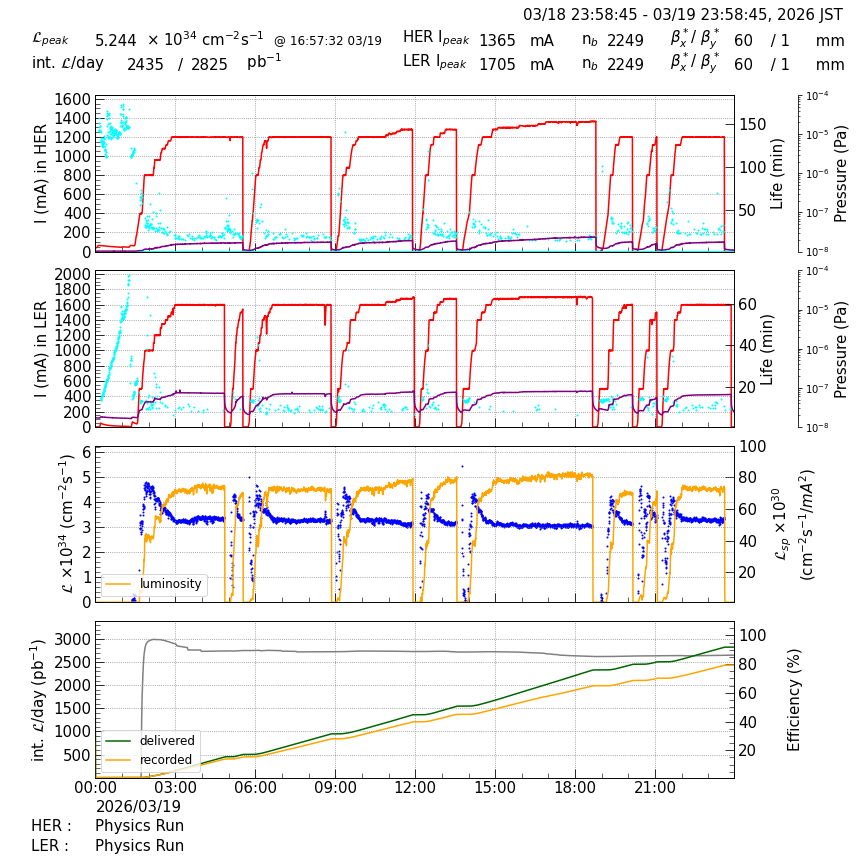
\includegraphics[width=0.8\textwidth]{belleII_det/images/SuperKEKB_operation.png}
\caption{SuperKEKB operating parameters on March 18-19, 2026. From top to bottom: HER and LER ring currents (first two panels), instantaneous and integrated luminosity (bottom two panels)}
\label{fig:SuperKEKB 24-Hour Operation Summary}
\end{figure}

\subsection{The Belle II detector}
The only interaction point of SuperKEKB is surrounded by the \textbf{Belle II} detector \cite{BelleIIPhysicsBook2019}, a general purpose high-energy particle layered detector with almost $4 \pi$ of solid angle coverage. It presents a cylindrical shape to cover the $e^+ e^-$ collisions, composed of a barrel and two end-caps located along the z-axis. 
$\\$
The Belle II detector measures 8 m in both width and height, with a total weight of approximately 1400 tons. With the exception of the KLM, all its subsystems are immersed in a 1.5 T magnetic field. 
$\\$
The detector is composed of several sub-detectors arranged cylindrically, reflecting the asymmetric distribution of the final state particles. The cylindrical structure of the detector is the \emph{barrel}, while the bases are made of the forward end-cap (along the direction of the $e^-$ beam) and the backward end-cap (along the direction of the $e^+$ beam). 
$\\$
The Belle II detector consists of the following sub-detectors, arranged radially outward from the IP:
\begin{enumerate}[label=(\alph*)]
\item Beam Pipe made of Beryllium (Be),
\item Two layers of silicon pixel detector (PXD),
\item Four layers of silicon strip detector (SVD),
\item The Central Drift Chamber for tracking the charged particle CDC, 
\item Time of propagation (TOP) Cherenkov counter in the barrel  + Cherenkov ring imaging (ARICH) in the front end-cap region,
\item The electromagnetic calorimeter (ECL) to detect photons and to identify charged particles, 
\item Superconductive magnet which provides 1.5 T axial magnetic field in order to bend charged particle, 
\item $K_L$ and muon detector (KLM) to track muons and $K_L$. 
\end{enumerate}

The electromagnetic calorimeter (ECL) has a central role in this elaborate since neutral ECL clusters associated to anti-neutron candidates are studied.
$\\$
A Belle II scheme is shown in ~\ref{fig:belleii_artistic}.

\begin{figure}[H]
    \centering
    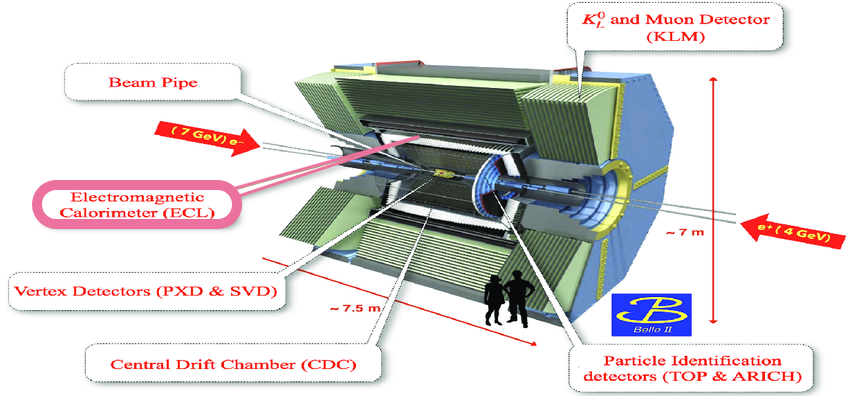
\includegraphics[width=1\textwidth]{belleII_det/images/belleii_dets}
    \caption{An artistic view of the Belle II detector}
    \label{fig:belleii_artistic}
\end{figure}

\subsubsection{The vertex detector VXD}
Immediately following the beryllium beam pipe, which does not play a detection role, the innermost layer is the Vertex Detector (\textbf{VXD}). 
$\\$
It consists of two devices: the Silicon Pixel Detector (\textbf{PXD} - 2 layers) \cite{YE2021164875} and the Silicon Vertex Detector (\textbf{SVD} - 4 layers) \cite{ZANI2022166952} . Overall there are six layers, of whose the first two ($r_1=14 mm, \ r_2=22 mm$) are pixelated sensors of the DEPFET type and the remaining four ($r_3=38 mm, \ r_4=88 mm, \ r_5=115 mm,\ r_6=140 mm$) are double-sided silicon strip sensors. 
$\\$
The VXD provides coverage of $17^\circ < \theta < 150^\circ$ and full azimuthal coverage in $\phi$, where $\theta$ is the polar angle relative to the $z$-axis -aligned with the $e^-$ beam direction- and $\phi$ is the azimuthal angle in the $xy$ plane using cylindrical coordinates.

\begin{figure}[H]
    \centering
    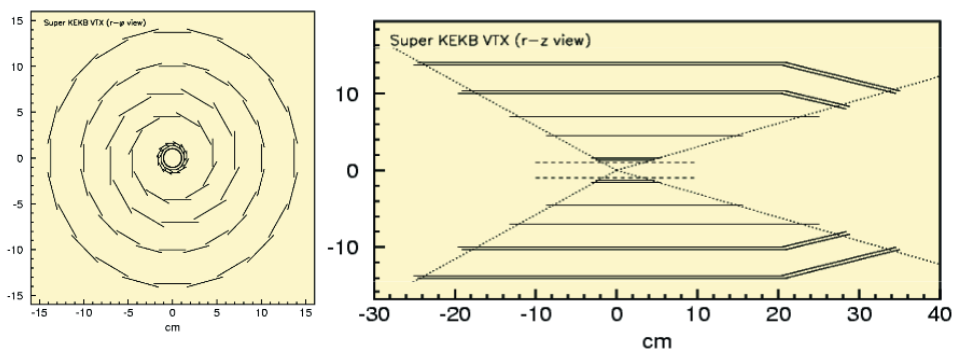
\includegraphics[width=0.95\textwidth]{belleII_det/images/VXD}
    \caption{A scheme of the Belle II VXD}
\end{figure}

The VXD purpose is to reconstruct the position of the primary vertex, the vertex of B-mesons decay which are directly produced by the decay of the $\Upsilon(4S)$, improving the resolution of the tracking system as well..

\subsubsection{The Central Drift Chamber (CDC)}
The Central Drift Chamber (\textbf{CDC}) is a large volume composed of small drift cells and it is the main tracking system of the Belle II detector, reconstructing charged-particle tracks by measuring the hit positions, which allows the determination of their momenta \cite{Taniguchi_2017}. Furthermore, the energy loss $\frac{dE}{dx}$ measure provides information for PID (Particle IDentification), thanks to the 1.5 T magnetic field. CDC has a radius of 1130 mm and it contains 14339 wires in total distributed in 56 layers, either parallel (axial orientation) or skewed (stereo orientation) to the longitudinal magnetic field . Combining their information, it is possible to reconstruct a full tridimensional helix track. Inside the cell, the average drift velocity is $3.3 \frac{cm}{\mu s}$. 
$\\$
The CDC has the same VXD angular ($\theta$, $\phi$) coverage and, in order to increase the forward acceptance, it is distributed asymmetrically along the z axis. It is filled with a mixture of $H_e C_2 \ (50\%)$ and $H_6 \ (50\%)$, which represents a good trade-off between a good momentum resolution for tracking and good $\frac{dE}{dx}$ resolution for the PID. A schematic view of the CDC is shown below:
\begin{figure}[H]
    \centering
    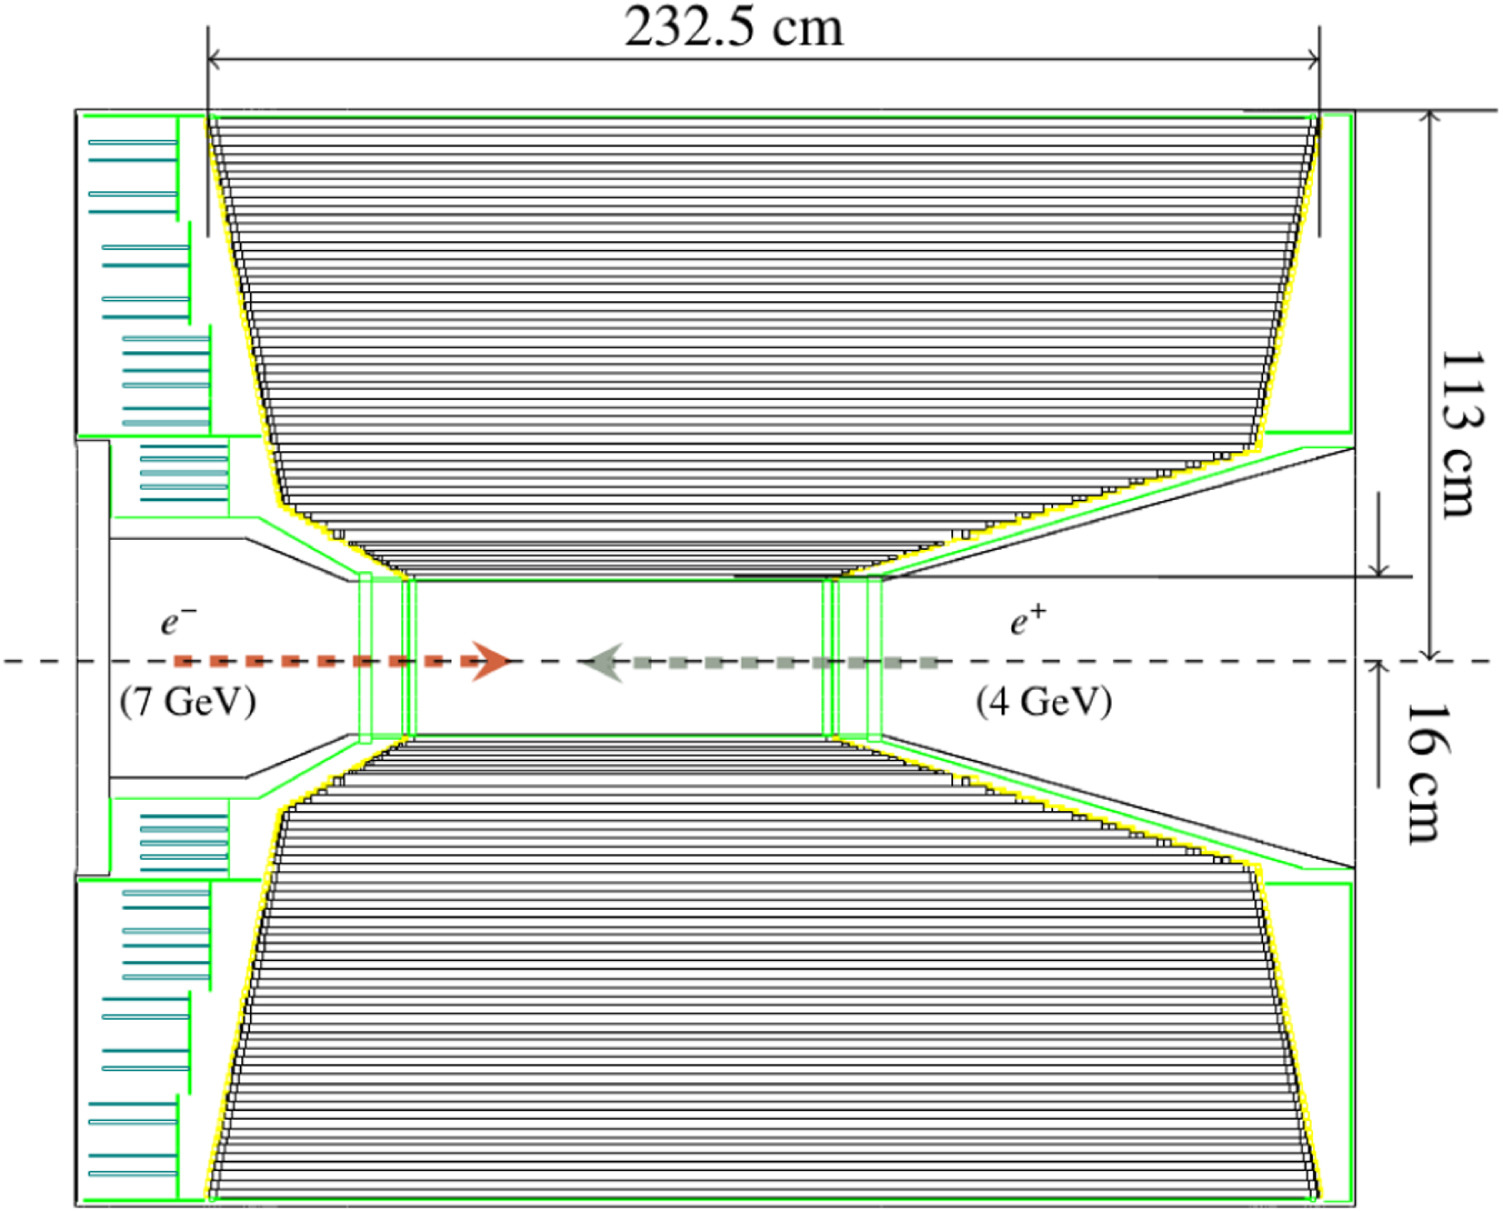
\includegraphics[width=1\textwidth]{belleII_det/images/CDC}
    \caption{A scheme of the Belle II CDC}
\end{figure}

\subsubsection{PID system: TOP and ARICH}
Particles crossing a Cherenkov radiator material with a speed $\beta > \frac{c}{n}$, where c is the speed of light and n is the material refractive indices, emit photons at an angle of $\theta_c = arcos(\frac{1}{\beta n})$.
$\\$
For Particle Identification in the barrel region, a Time of Propagation (\textbf{TOP}) counter is employed. It is a novel type of Cherenkov detector \cite{Horii:2013ndq} used for particle identification in the barrel region. In total, there are 16 modules, each consisting of a 45 cm wide and 2 cm thick quartz bar with a small expansion volume of about 10 cm long at the sensor end. There is an expansion wedge that behaves as a lens and improves the spatial resolution of the Cherenkov photon imaging. At the exit window of the wedge, two rows of sixteen fast multi-anode photon detectors are mounted.
$\\$
Within the 2.6 m-long quartz the particle produces Cherenkov radiation that travels via total internal reflection to the mirror, where they are reflected towards the photon detectors at the backward end, where is located a small prism which serves as a volume expansion and a light guide. The time of arrival and the impact position of the Cherenkov photons provide the 2D Cherenkov ring signal. 
$\\$
The hit distributions differ according to the particle species and their masses: different particles exhibit distinct Cherenkov angles, resulting in different photon paths. Consequently, they are detected at different positions within the PMT array and at different times.


\begin{figure}[h]
    \centering
    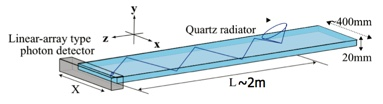
\includegraphics[width=0.8 \textwidth]{belleII_det/images/top}
    \caption{Scheme of TOP counter module}
\end{figure}

\begin{figure}[h]
    \centering
    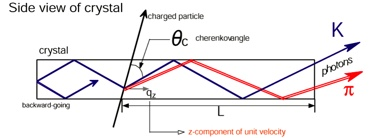
\includegraphics[width=0.8 \textwidth]{belleII_det/images/top2}
    \caption{Representation of the side view of TOP counter with internal reflection of the Cherenkov radiation}
\end{figure}

Thanks to a 16-channel Micro Channel Plate PhotoMultiplier (MCP-PMT), TOP counters are equipped with photosensors that provide a time resolution of about 100 ps.
$\\$
The Aerogel Ring Imaging CHerenkov (\textbf{ARICH}) \cite{Yusa:2013cao} is located in the forward end-cap region of the Belle II detector and is thus complementary to the aforementioned TOP. Its main goal is to separate kaons $K$ from pions $\pi$ across the full kinematic range of the experiment, from 0.5 to 4.0 $GeV/c$.
$\\$
Since particles with the same momentum but different mass radiate at different angles, it is designed to detect and distinguish forward-going charged particles. It consists of two 2 cm thick layers of aerogel ($n_{up} = 1.045, n_{down} = 1.055$), which increase the photon yield without degrading the Cherenkov angle resolution.

\begin{figure}[H]
    \centering
    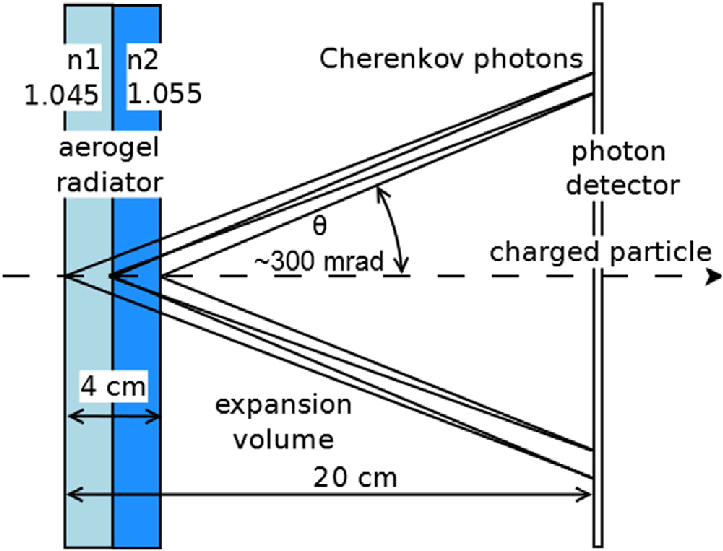
\includegraphics[width= 0.49\textwidth]{belleII_det/images/ARICH}
    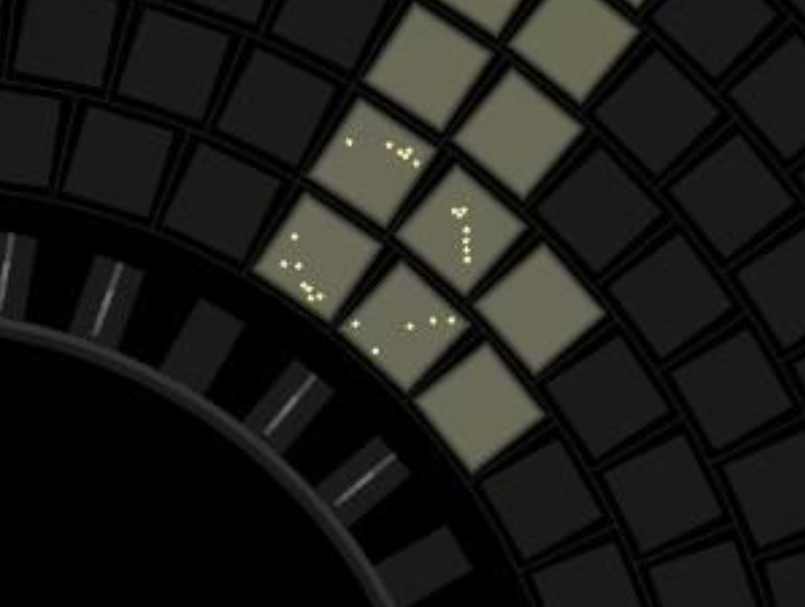
\includegraphics[width= 0.49\textwidth]{belleII_det/images/mu_ring}    
    \caption{(a) working principle of ARICH (b) ring produced by a cosmic muon}
    \label{fig:mesh2}
\end{figure}

\subsubsection{The Electromagnetic Calorimeter (ECL)}
The Electromagnetic CaLorimeter (\textbf{ECL}) plays a central role in this thesis, since the neutral ECL clusters associated to anti-neutron candidates are studied.
$\\$
A calorimeter is a detector designed to measure particle energy. As particles enter, they initiate electromagnetic or hadronic showers, depositing their energy within the detector material, which is then collected and precisely measured. 

\begin{figure}[h]
    \centering
    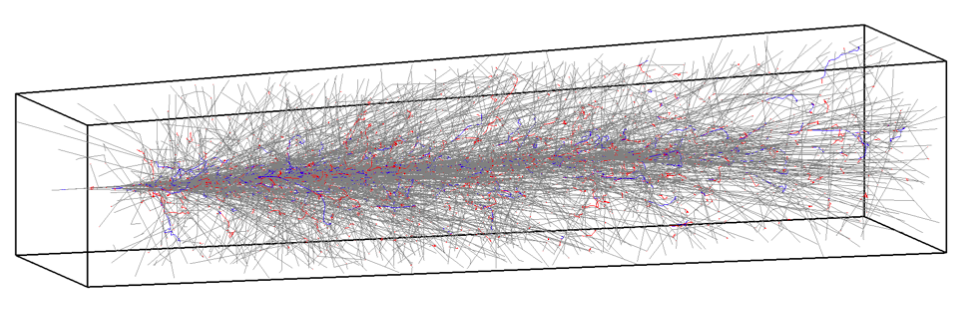
\includegraphics[width=0.95\textwidth]{belleII_det/images/shower_ECL}
    \caption{Typical ECL shower caused by a 7 GeV photon}
\end{figure}

However, as its name suggests, the primary aim of the ECL is to detect photons and electrons, providing precise measurements of the energy and position ($E$, $\vec{x}$) of electromagnetic showers \cite{KUZMIN2020162235}. It must identify neutral particles, such as photons and neutral hadrons, as well as charged ones (mostly electrons and pions). Anti-neutron is detected through its annihilation products (mainly pions), as previously discussed.
$\\$
The Molière radius $R_m$ is defined as 
\begin{center}
$R_m = \frac{21 MeV}{E_c} \times X_0$, where $E_c$ is the material critic energy
\end{center}
The rule of thumb for electromagnetic calorimeter is that $\sim 90\%$ of electromagnetic shower is contained in a cylinder with radius $R_m$, while the $\sim 95\%$ is contained in a cylinder with radius $2R_m$.

\paragraph{CsI(Tl) crystals}
$\\$
The thallium-doped caesium iodide \textbf{CsI(Tl)} crystals have $X_0$ = 1.860 cm and $R_m$ = 3.53 cm. This material is one of the brightest known scintillator, providing a light yield Y of  $\sim 52000$ photons/MeV, with a photon emission spectrum at $\sim 550$ nm, ideal for photodiode readout. 

\begin{figure}[H]
    \centering
    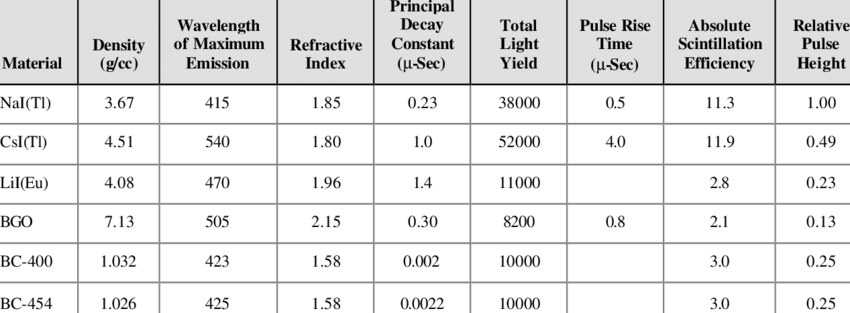
\includegraphics[width=1\textwidth]{belleII_det/images/Properties-of-scintillators}
    \caption{Properties of inorganic scintillators used in calorimetry \cite{nedilko2009}}
\end{figure}

The ECL is composed of 8736 array of \textbf{CsI(Tl)} crystals. Each is a truncated pyramid with dimension 6x6x30 $cm^3$, where the radial length is around 16.2$X_0$. Each crystals is wrapped with a layer of 200  $\mu m$ thick Gore-Tex porous teflon and then covered with a 50 $ \mu m$ thick aluminized polyethylene.
$\\$
The ECL is made of a 3 m long barrel section and the end-caps at $z = 2.0$ m (forward) and $z = -1.0$ m (backward). An ECL scheme is shown below:

\begin{figure}[H]
    \centering
    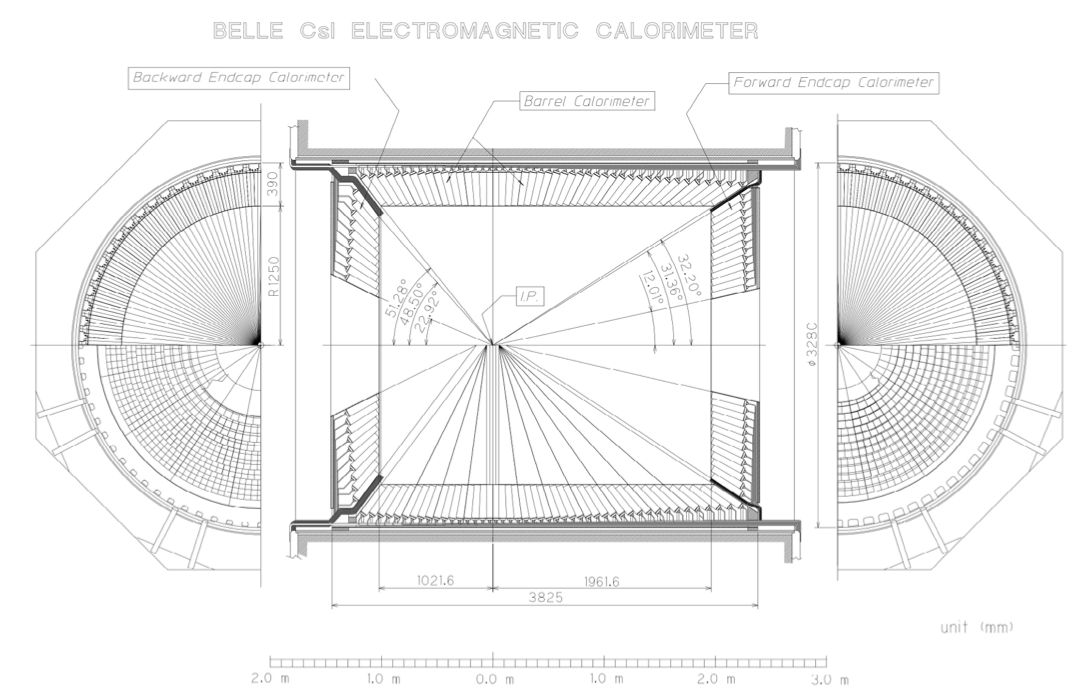
\includegraphics[width=1\textwidth]{belleII_det/images/ECL}
    \caption{A scheme of the Belle II ECL detector}
\end{figure}

It then is located in the barrel region and in the forward/backward end-cap region too, covering about 90\% of the solid angle in the center-of-mass system (polar coverage: $12^{\circ} \le \theta \le 155^{\circ}$); two $\sim1^{\circ}$ gaps between barrel and end-caps.
$\\$
Lights coming from each crystals is detected by two $10 \times 20 mm^2$ \emph{Hamamatsu S2744-08} photodiodes glued to the rear surface of the crystals and coupled with charge-sensitive pre-amplifiers.

\begin{figure}[H]
    \centering
    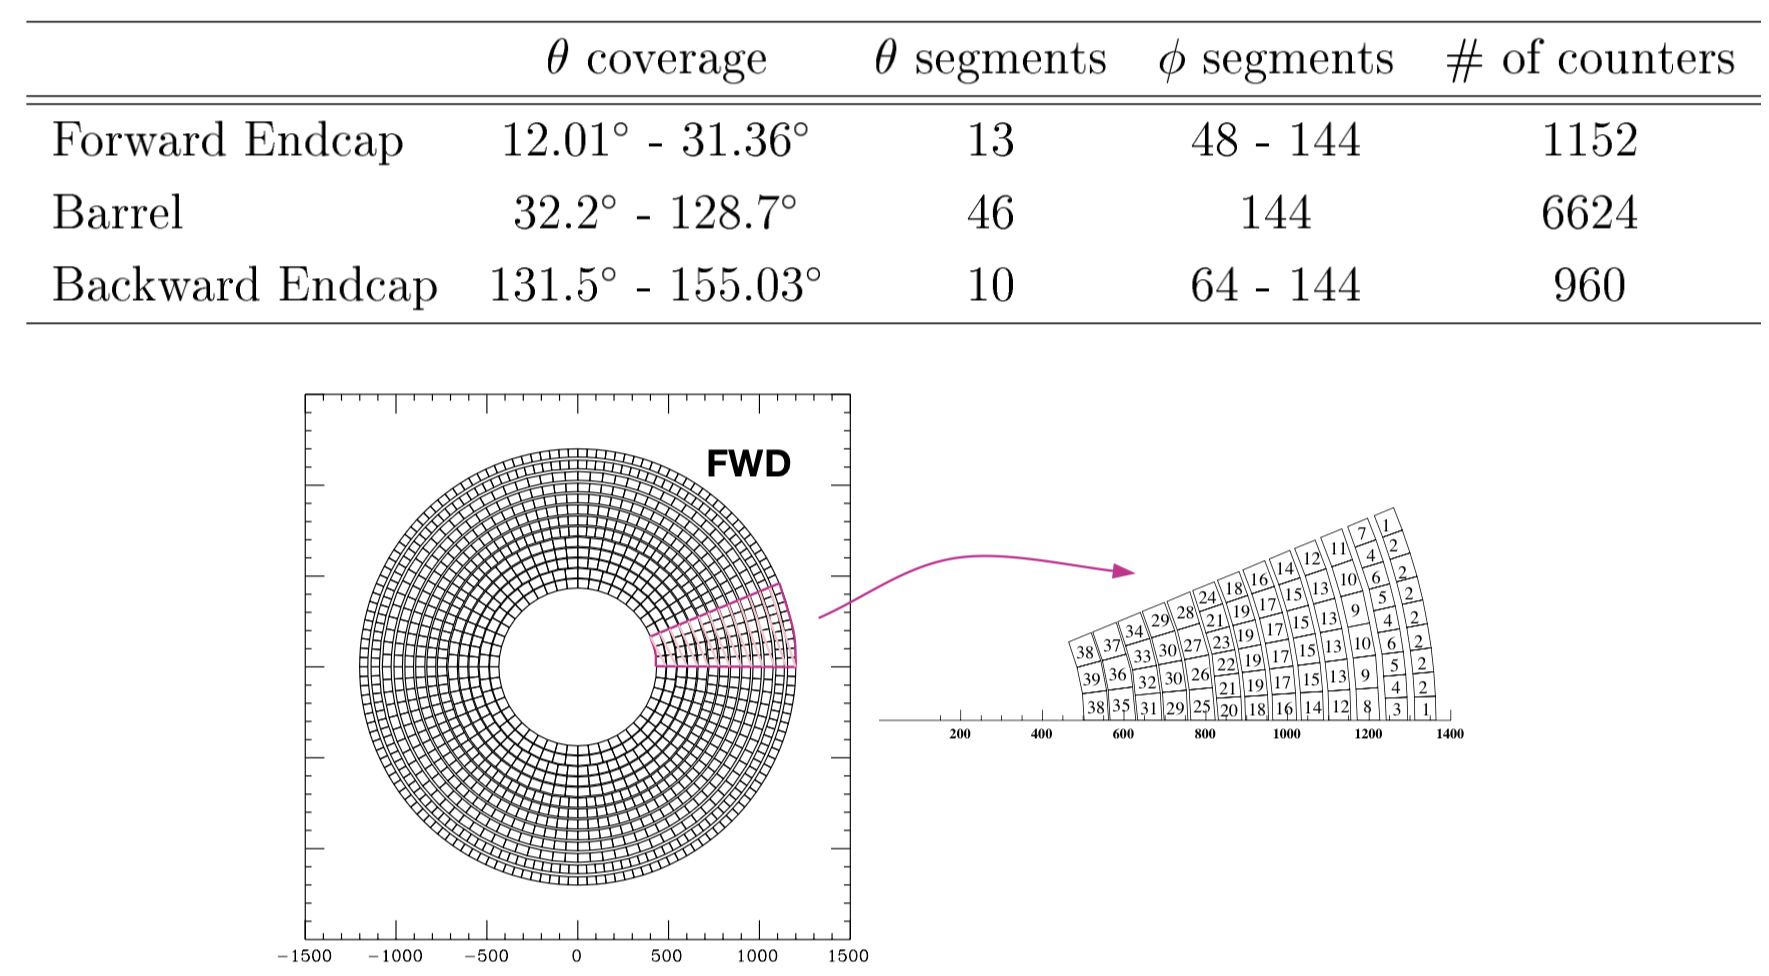
\includegraphics[width=0.85\textwidth]{belleII_det/images/ECL_division}
    \caption{ECL coverage and segmentation}
\end{figure}

\paragraph{The ECL  reconstruction algorithm} 
$\\$
as mentioned, the main tasks of an electromagnetic calorimeter are to measure the energy and position of electromagnetic showers and to identify neutral and charged particles. For each crystals, a 32 bit word is the result of the signal, namely an \textbf{ECLDigit}. It is made of the energy information in GeV (18 bit), the time information in ns (12 bit) and 2 status bits (quality of the signal). In order to reconstruct the shower, there is an algorithm which converts the ECLDigit into ECLShowers and the into ECLClusters.
$\\$
The first step is to identify the  \textbf{connected regions}, which allows a rapid reduction of the combinatorics. An example of this procedure is shown below:

\begin{figure}[H]
    \centering
    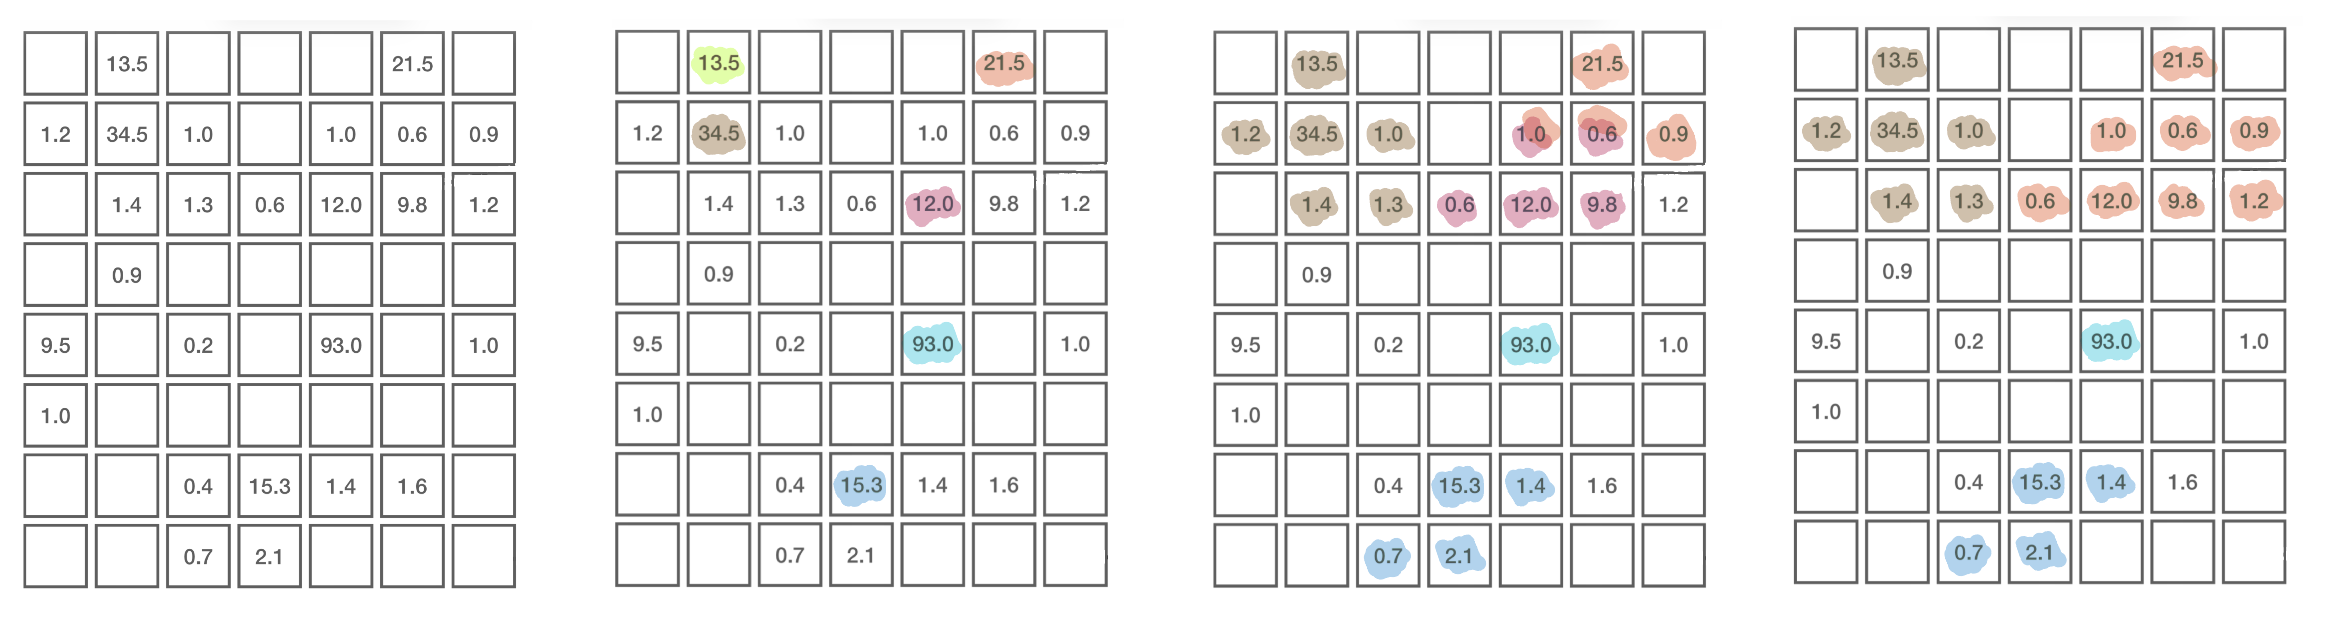
\includegraphics[width=1\textwidth]{belleII_det/images/ECL_algo}
  \caption{Description of ECL clustering process:(a) Step 0 (b) Step 1 (c) Step 2 (d) Step 3}
\end{figure}

Each cell represents one ECLDigit, whose value corresponds to the energy in MeV. Empty cells are below the readout threshold (0.1 MeV for this example). In step 1, every ECLDigit above 10 MeV is selected. In step 2, any neighbors above 0.5 MeV are attached to the highest-energy seed found in step 1. Sometimes two seeds compete for the same neighbor, and sometimes clusters have no neighbors (i.e. 93.0). In step 3, overlapping neighbor regions trigger a merge. Additionally, any cells above 1.5 MeV recruit their next neighbors iteratively.
$\\$
After this process, the connected regions are obtained:

\begin{figure}[H]
    \centering
    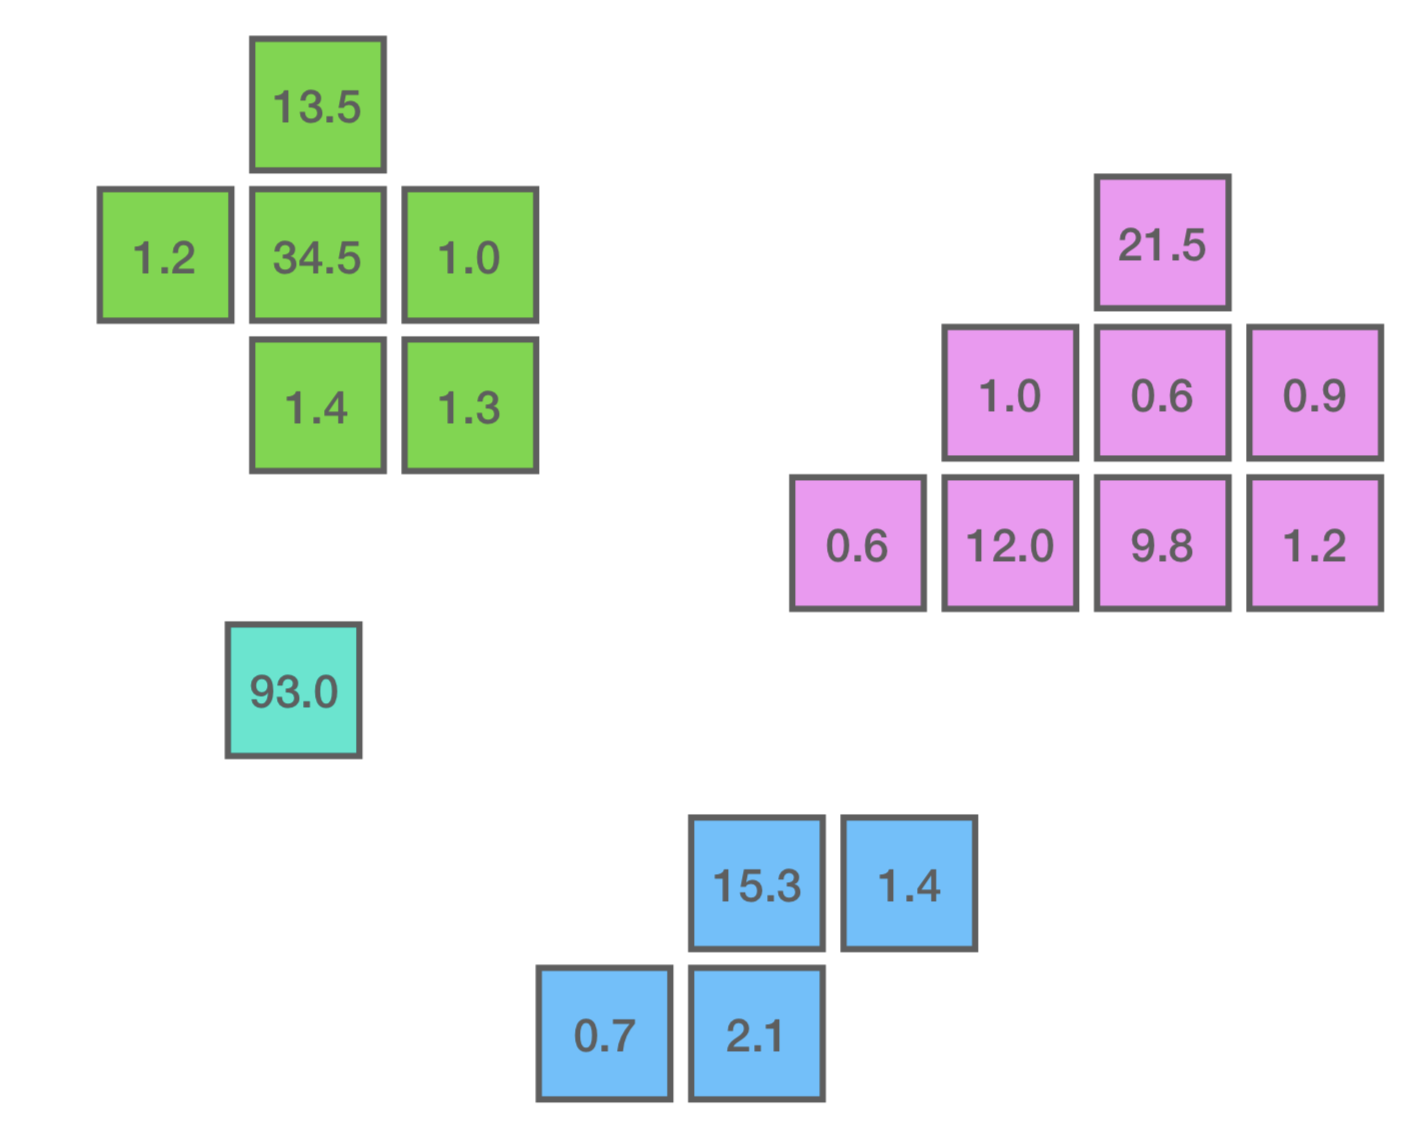
\includegraphics[width=0.5\textwidth]{belleII_det/images/ConnectedRegions}
\end{figure}
The final step is to pick the crystals with energy above 10 GeV, namely the Local Maxima (LM). Every connected region has one LM at least. The connected regions are furtherly processed in order to obtain the position and the energy of the cluster, processing the LM with a splitting-weighting process among the connected regions crystals \cite{denuccio2019}. 
$\\$
The main idea is that an \textbf{ECLShower} object is produced from every LM. If there is only one local maximum within a connected region, the full energy of each crystal is associated with the corresponding ECLShower. Otherwise, if multiple local maxima are present, an iterative procedure is performed, where the weight for each crystal depends on the distance of the crystal from the center-of-gravity of each ECLShower (enter-of-gravity is calculated using weighted energies).
$\\$
Connected regions are used to minimize the number of times the computationally intensive splitting procedure must be performed.

\paragraph{ECL performance}
$\\$
The observed ECL \textbf{energy resolution} can be written as follow:
\begin{center}
$\sigma_E = \sqrt{ \left( \frac{0.81\%}{\sqrt[4]{E}} \right)^2 + \left( \frac{0.066\%}{E} \right)^2 + (1.34\%)^2 }$
\end{center}
Where the first term represents stochastic fluctuations (Poissonian statistics) in shower generation, the second term accounts for electronic noise, and the third is a constant term dependent on calibration.
$\\$
For example, $\frac{\sigma_E}{E} = 4\%$ at 100 MeV and $\frac{\sigma_E}{E} = 1.4\%$ at 8 GeV, while the angular resolution is 13 mrad (3 mrad) at low (high) energies. For example, the $\pi^0$ mass is 135 MeV and its mass resolution is approximately 4.5 MeV, in absence of background (detailed description can be found in \cite{abashian2002}).

\begin{figure}[H]
    \centering
    \includegraphics[width=1\textwidth]{belleII_det/images/energy-res}    
\end{figure}

\begin{figure}[H]
    \includegraphics[width=1\textwidth]{belleII_det/images/energy-res2}
  \caption{The energy resolution as a function of incident photon energy for the (a) 3Y3 and (b) 5Y5 matrix with total energy sum. The energy resolution of the (c) 3Y3 and (d) 5Y5 matrix with a 0.5 MeV threshold. The solid lines are the results of the "t. The error bars are not statistical but are the rms of four measurements taken with the crystals (3,3), (3,4), (4,3) and (4,4) into the photon beam \cite{ikeda2000belle}}
\end{figure}


\subsubsection{Solenoid and iron structure} 
Following the ECL, an axial magnetic field of 1.5T is generated by a 23 tons superconducting solenoid. The curvature of charged-particle trajectories (Larmor radius) allows the determination of their momentum and charge, which, when combined with additional detector information, enables particle identification.
$\\$
It is made of niobium-titanium-copper (NbTi/Cu) alloy and it is cooled by liquid helium cryostat in order to reach superconducting conditions.
\subsubsection{The $K_L$ and Muon Detector (KLM)}
Following the solenoid, the \textbf{KLM} detector represents the outermost layer of Belle II and it is dedicated to the detection of $K_L$ mesons and muons, which are very penetrating particles. It is composed of alternating layers of 4.7 cm thick iron plates and active detector elements; the former acts as a return yoke for the magnetic flux. They also provide at least 3.9 interaction lengths (compared to 0.8 in the ECL), allowing the $K_L$ to interact and produce hadronic showers.
$\\$
KLM covers the barrel region (15 layers) and the end-caps regions (forward 14 layers and backward 12 layers). The two inner barrel layers and the entire end-caps are instrumented with scintillator strips, while the 13 outer barrel layers are instrumented with Resistive Plate Chambers (RPC). 
$\\$
As compared to charged hadrons, muons travel longer distances and with smaller deflections inside the KLM, which allows discrimination between the two.

\subsection{The Belle II Analysis Software Framework}
\begin{figure}[H]
    \centering
    
\includegraphics[width=0.4\textwidth]{belleII_det/images/b2logo}
\end{figure}

To perform the simulations, reconstruction and the analyses of this thesis, the Belle II Analysis Software Framework (\textbf{basf2}) has been employed. It is the primary software used in all aspects of the online data-processing chain at Belle II, such as generating simulated data, unpacking raw data, performing reconstruction (tracking, clustering) and carrying out high-level analysis. The final analysis steps (the Offline Analysis as histogramming, fitting distributions, etc.) are usually performed in other frameworks as well, such as \textbf{ROOT} or the Matplotlib Python library.

\subsubsection{Monte Carlo method}
The Monte Carlo method is a technique used to compute probabilities and related quantities by exploiting sequences of pseudo-random numbers. Sequences of random numbers possess meaning, not individual ones—though the latter are frequently referenced. Randomness characterizes the sequence, not single numbers. 

\paragraph{Simulation}
$\\$
Monte Carlo methods are widely used in HEP physics for tasks such as \textbf{event generation simulation} and \textbf{detector simulation}. The first one regards the production and the decays of particles with a certain set of properties, while the second one concerns the simulation of the particle interactions during the path in the detector materials. After the electrons and positrons collision, a certain amount of particles are produced according to the adopted physical model, that could follow either the Standard Model or more advanced ones, such as super symmetry or dark matter production ones. Example of those could be \emph{PYTHIA} for the generation of high-energy physics collision events, \emph{EvtGen} that simulates the decays of heavy flavour particles, primarily B and D mesons and \emph{Phokhara} which simulates the leptonic and hadronic final states at the next-to-leading order (NLO) accuracy, namely simulating ISR radiation, which will have a primary role in the next chapters, and so forth.
$\\$
After particle generation, the simulation of propagation through the detector must be addressed, including interactions with active materials and the material budget. This is powered \emph{GEANT4}, an open source software which performs the interaction between particles and the detector systems. The materials of the detectors are specified by their physical features, like atomic number, mass number and density via ROOT geometry class \emph{TGeoManager}.

\begin{figure}[H]
    \centering
    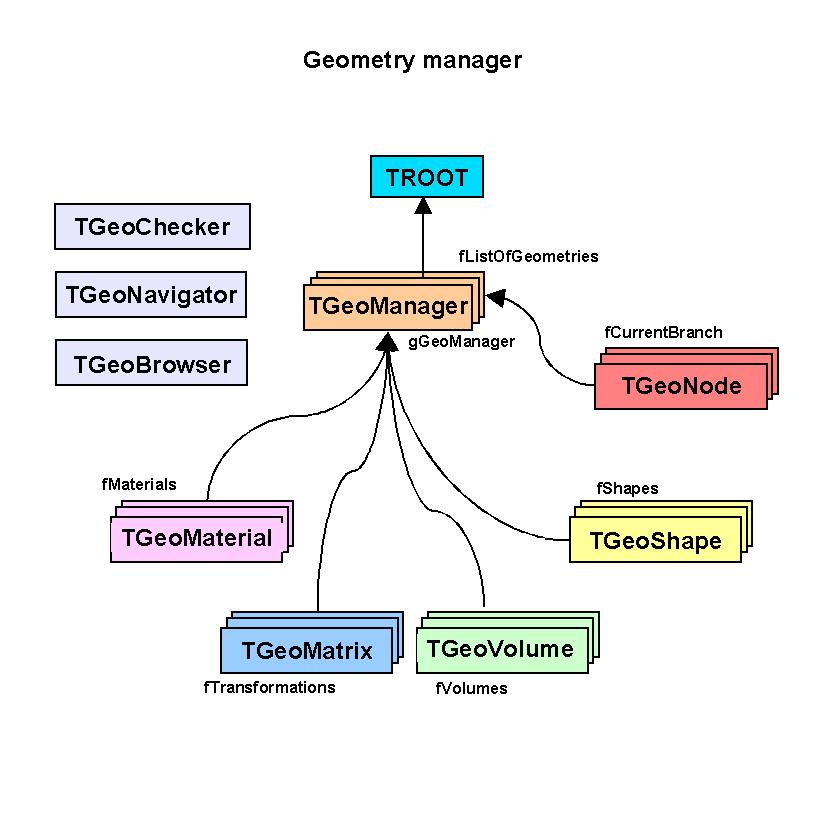
\includegraphics[width= 0.40\textwidth]{belleII_det/images/TGeoManager}
    \caption{TGeoManager Class Diagram}
\end{figure}

\paragraph{Reconstruction}
$\\$
The reconstruction process allows the particles measurement and identification. The closer the reconstructed quantities (such as initial positions and four-momenta) are to the generated-level information, the better the reconstruction performance in simulated MC and real data. Since several products of $e^+ e^-$ are short living particles, it is necessary to reconstruct them indirectly via their daughter particles. Furthermore, intrinsic noise must be taken into account, as it may generate spurious random signals unrelated to actual particles. Interactions between beam electrons or positrons, either with each other or with other accelerator components -known as beam background- must be considered.
$\\$
The same reconstruction algorithms are employed in data and MC, in order to obtain the same reconstruction: in order to test the correct response of the reconstruction, the so called \textbf{MCTruth} are use used, which basically is the generator-level Monte Carlo truth of the simulated data pool. The Monte Carlo matching (MC-matching) procedure identifies the generator-level particle responsible for a reconstructed candidate, crucial for understanding reconstruction effects and backgrounds. This corresponds to the association of reconstructed particles with MC particles in Belle II nomenclature.

\subsubsection{basf2 modules and path}
A \textbf{basf2 module} is the smallest building block of the framework and it is a script, usually written in C++, designed to process a specific unit of data. A typical data chain consists of a linear arrangement of modules. All the work is done in modules, including reading and writing data to and from disk or more complex operations such as full detector simulation.
$\\$
Modules are linearly arranged in a \textbf{path}, which is a container for them. The linear order depends on the specific task defined by the user. Therefore, the modules are executed one at a time, in the same order they were added into the path, from the first to the last. A schematic view of processing flow is shown below:

\begin{figure}[H]
    \centering
    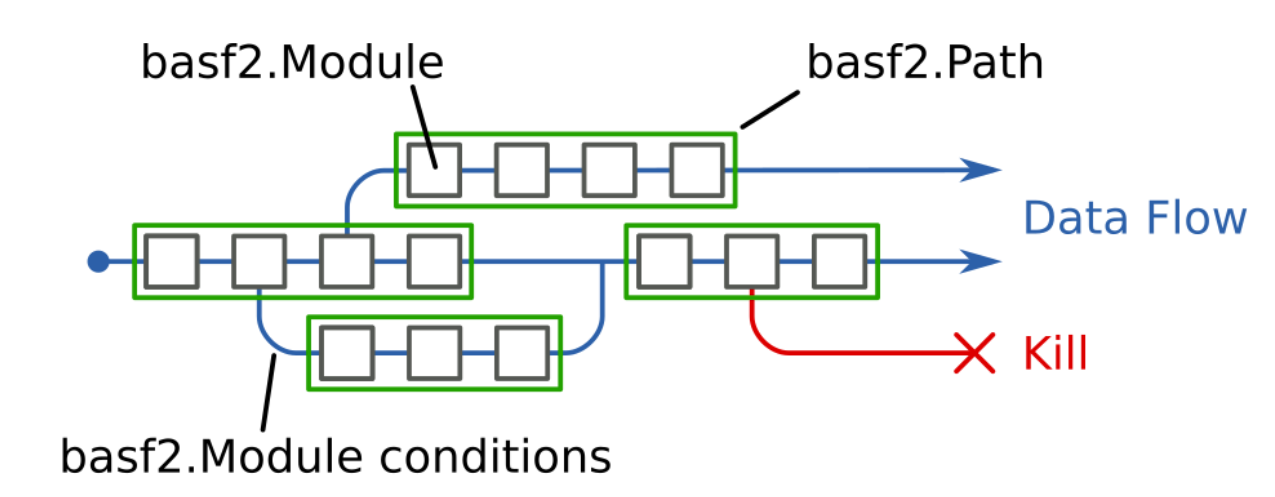
\includegraphics[width= 0.70\textwidth]{belleII_det/images/basf2_1}
    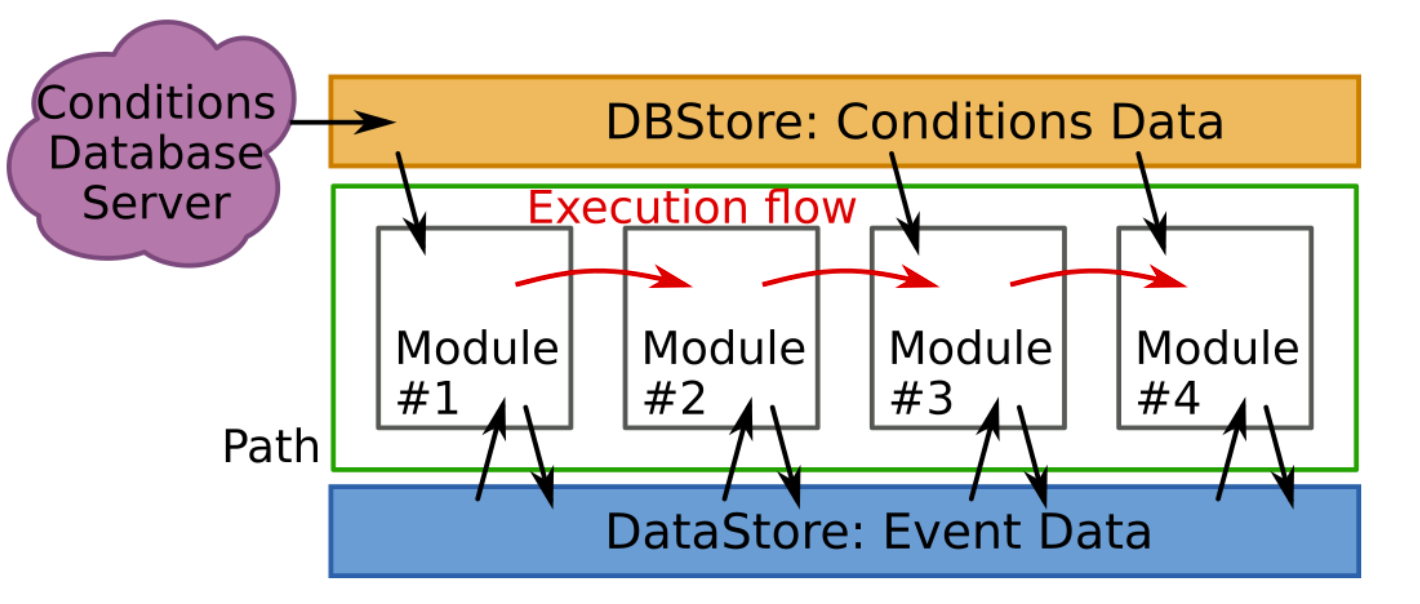
\includegraphics[width= 0.70\textwidth]{belleII_det/images/basf2_2}    
    \caption{Scheme of the processing chain in basf2}
\end{figure}

The modules process data stored in the DataStore, with each module having access to read from and write to it. There is also a non-event data, the so called conditions, which is loaded from a central conditions database and is available in the DBStore. These databases stores the information about the specific detector condition at each run of the experiment. 

A \textbf{package} is a logical collection of code in basf2, consisting of several modules and some python scripts that configure paths to do common things. The packages have meaningful name related to their specific operation (tracking, reconstruction, ecl, klm, etc...). All the packages are stored in the Belle II GitLab directory. The most used package in this thesis is the \textbf{analysis package}, which contains python functions and C++ basf2 modules, such as modularAnalysis.
$\\$
The \textbf{steering file} is the core script in which analysis and data-processing tasks are performed, with a path being declared and modules added to it. Some highlights of the steering files used are provided in the appendix.

\subsubsection{TopoAna: Topology Analysis}
In high-energy physics data analysis, a comprehensive understanding of inclusive MC samples could be crucial to select signals with higher efficiency while suppressing backgrounds. This is exactly the case of the present elaborate. 
$\\$
Knowledge of the physics processes enables identification of the main backgrounds. Selection criteria can then be further optimized by analyzing differences between these backgrounds and the signal. 

\begin{figure}[H]
    \centering
    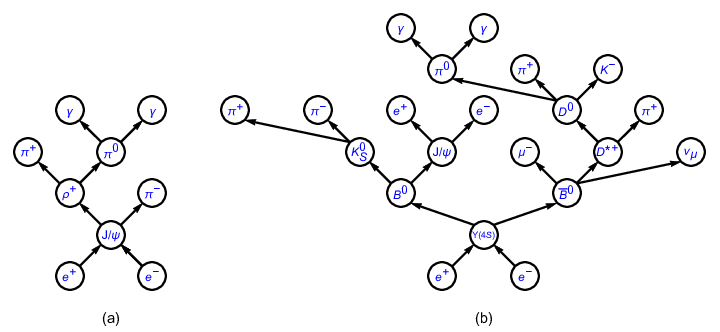
\includegraphics[width= 0.95\textwidth]{belleII_det/images/topology_diagrams}
    \caption{Topology diagrams of (a) $e^+e^-\rightarrow J/\psi$ and (b) $ e^+e^-\rightarrow \Upsilon(4S)\to B^0 \bar{B}^0$, two typical processes at $e^+ e^-$ colliders, such as Belle II and BESIII}
    \label{fig:topoproc}
\end{figure}

In order to have a very quick way to verify the Monte Carlo quickly and easily, a topology analysis program called \textbf{TopoAna} is developed with C++, ROOT, and LaTeX.
$\\$
The program input consists of one or more ROOT files containing a \textbf{TTree} object with raw topology truth information from the inclusive MC samples under study. Specifically, each \textbf{TTree} entry includes three key ingredients for particles produced in an event: the particle multiplicity, their PDG codes, and their mother indices.
$\\$
TopoAna is an offline tool independent of basf2. It independently extracts human-readable topology information from raw MC truth data via the MCGenTopo interface. Referring to figure ~\ref{fig:topoproc} (b):
\begin{figure}[H]
    \centering
    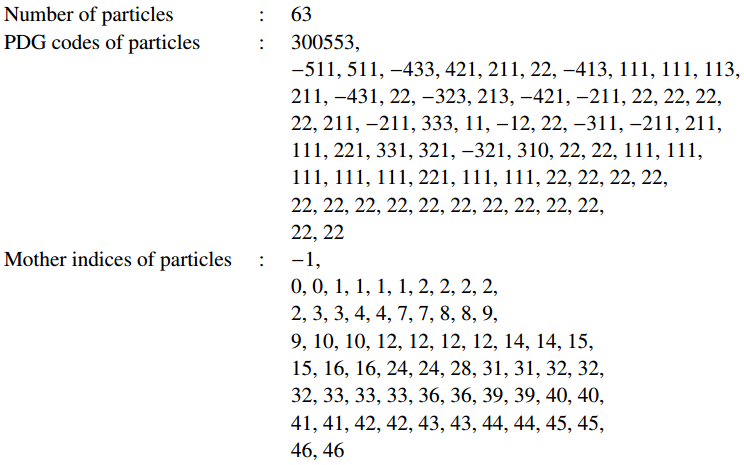
\includegraphics[width= 0.49\textwidth]{belleII_det/images/topology_diagrams_2}
     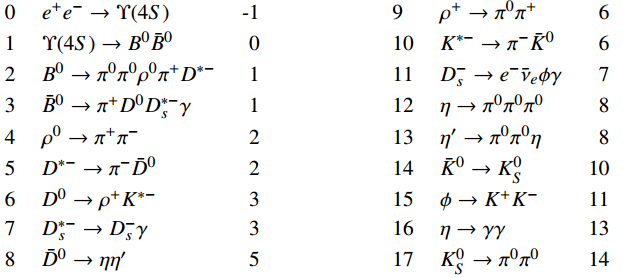
\includegraphics[width= 0.49\textwidth]{belleII_det/images/topology_diagrams_3}
    \caption{(a) Raw and (b) highly readable symbolic expressions of physics processes ~\ref{fig:topoproc} (b):}
\end{figure}

